\documentclass[aspectratio=169,11pt]{beamer}
\usetheme{Madrid}
\usecolortheme{seahorse}
\usepackage[T1]{fontenc}
\usepackage[utf8]{inputenc}
\usepackage{booktabs}
\usepackage{tikz}
\usetikzlibrary{arrows.meta,positioning,shapes.geometric}

\setbeamertemplate{navigation symbols}{}
\setbeamertemplate{footline}[frame number]

\title{Labyrinth Breach -- Implementation Deep Dive}
\subtitle{System Architecture, Code Walkthrough \& Live Demo}
\author{Ahmed Jawed}
\institute{AI641 -- AI for Robotics | MS AI, LUMS}
\date{May 2025}

\begin{document}

% ============================================================
\begin{frame}
\titlepage
\end{frame}

% ============================================================
\begin{frame}{What I Will Cover}
\begin{enumerate}
\item \textbf{System Architecture} -- how the pieces connect
\item \textbf{Observation Pipeline} -- how agents see the world
\item \textbf{Reward Engine} -- how we shape behavior
\item \textbf{Training Pipeline} -- curriculum \& config flow
\item \textbf{Logging \& Evaluation} -- how we measure results
\item \textbf{Live Demo} -- trained agents in the dynamic maze
\end{enumerate}
\end{frame}

% ============================================================
\begin{frame}{System Architecture Overview}
\begin{center}
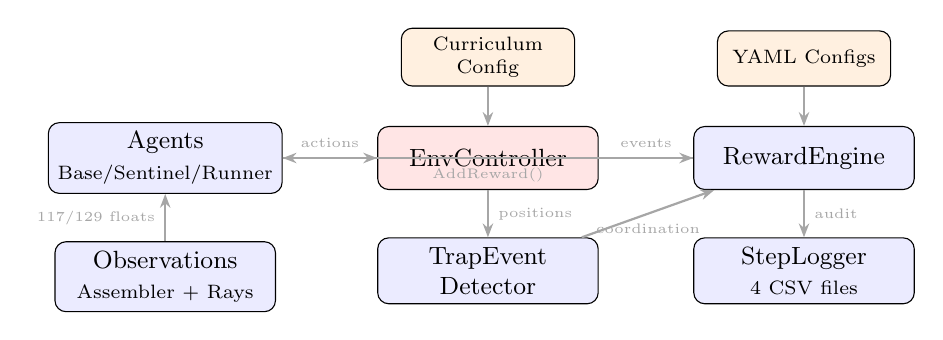
\begin{tikzpicture}[
  box/.style={draw, rounded corners, fill=blue!8, minimum width=2.8cm, minimum height=0.8cm, align=center, font=\small},
  configbox/.style={draw, rounded corners, fill=orange!12, minimum width=2.2cm, minimum height=0.7cm, align=center, font=\scriptsize},
  arrow/.style={-{Stealth[length=5pt]}, thick, color=gray!70},
  node distance=0.6cm and 0.8cm
]
  % Main components
  \node[box, fill=red!10] (ctrl) {EnvController};
  \node[box, left=1.2cm of ctrl] (agents) {Agents\\{\scriptsize Base/Sentinel/Runner}};
  \node[box, right=1.2cm of ctrl] (reward) {RewardEngine};
  \node[box, below=of agents] (obs) {Observations\\{\scriptsize Assembler + Rays}};
  \node[box, below=of ctrl] (trap) {TrapEvent\\Detector};
  \node[box, below=of reward] (log) {StepLogger\\{\scriptsize 4 CSV files}};
  
  % Config
  \node[configbox, above=0.5cm of reward] (yaml) {YAML Configs};
  \node[configbox, above=0.5cm of ctrl] (curriculum) {Curriculum\\Config};
  
  % Arrows
  \draw[arrow] (agents) -- (ctrl) node[midway,above,font=\tiny] {actions};
  \draw[arrow] (ctrl) -- (reward) node[midway,above,font=\tiny] {events};
  \draw[arrow] (reward) -- (agents.east|-reward) node[midway,below,font=\tiny] {AddReward()};
  \draw[arrow] (obs) -- (agents) node[midway,left,font=\tiny] {117/129 floats};
  \draw[arrow] (ctrl) -- (trap) node[midway,right,font=\tiny] {positions};
  \draw[arrow] (trap) -- (reward) node[midway,below,font=\tiny] {coordination};
  \draw[arrow] (reward) -- (log) node[midway,right,font=\tiny] {audit};
  \draw[arrow] (yaml) -- (reward);
  \draw[arrow] (curriculum) -- (ctrl);
\end{tikzpicture}
\end{center}
\vspace{-4pt}
{\small\textbf{Key design:} Everything is config-driven. Change reward weights, curriculum thresholds, or observation setup without touching C\# code.}
\end{frame}

% ============================================================
\begin{frame}{Agent Hierarchy}
\begin{columns}[T]
\column{0.5\textwidth}
\textbf{Inheritance Chain}
\begin{itemize}
\item \texttt{Unity.MLAgents.Agent}
  \begin{itemize}
  \item \texttt{BaseAgent} -- movement, observation collection, ML-Agents hooks
    \begin{itemize}
    \item \texttt{SentinelAgent} -- capture radius, target tracking
    \item \texttt{RunnerAgent} -- escape logic, captured state
    \end{itemize}
  \end{itemize}
\end{itemize}

\vspace{6pt}
\textbf{Parameter Sharing}
\begin{itemize}
\item All 3 Sentinels $\rightarrow$ one PPO brain
\item Both Runners $\rightarrow$ one PPO brain
\item Same weights, different observations
\item What one agent learns, all agents know
\end{itemize}

\column{0.5\textwidth}
\textbf{ML-Agents Lifecycle (every step)}
\begin{enumerate}
\item \textbf{Observe} -- \texttt{CollectObservations} builds the 117/129 float vector from sensors, rays, and memory
\item \textbf{Decide} -- neural network maps observation $\rightarrow$ 2 continuous actions (moveX, moveZ)
\item \textbf{Act} -- \texttt{OnActionReceived} applies movement to the agent's rigidbody
\item \textbf{Reward} -- \texttt{RewardEngine} computes and assigns reward
\item \textbf{Log} -- \texttt{StepLogger} records the event to CSV
\end{enumerate}

\vspace{6pt}
\textbf{Episode boundaries}
\begin{itemize}
\item Start: agents reset position and memory
\item End: both Runners captured, Runner reaches exit, or 120s timeout
\end{itemize}
\end{columns}
\end{frame}

% ============================================================
\begin{frame}{Observation Pipeline -- How Agents See}
\begin{columns}[T]
\column{0.55\textwidth}
\begin{tabular}{@{}lcc@{}}
\toprule
\textbf{Component} & \textbf{Sent.} & \textbf{Run.} \\
\midrule
Self state & 10 & 10 \\
Env context & 7 & 7 \\
Rays ($N \times 6$) & 84 & 96 \\
LOS memory & 6 & 6 \\
Opponent summary & 10 & 10 \\
\midrule
\textbf{Total} & \textbf{117} & \textbf{129} \\
\bottomrule
\end{tabular}

\vspace{8pt}
\textbf{Each ray = 6 floats:}
\begin{enumerate}
\item Normalized hit distance
\item Wall (one-hot)
\item Exit zone (one-hot)
\item Teammate (one-hot)
\item Opponent (one-hot)
\item Other object (one-hot)
\end{enumerate}

\column{0.45\textwidth}
\textbf{Design Decisions}
\begin{itemize}
\item \textbf{No camera/pixels} -- vector observations train 10x faster and are fully interpretable
\item \textbf{No global state} -- agents never see the full maze, making this a true POSG
\item \textbf{Memory} -- stores last-known XYZ when target leaves LOS, decays over time
\item \textbf{Opponent summary} -- 2 nearest enemies: distance, relative position, visibility, threat pressure
\end{itemize}

\vspace{6pt}
\textbf{Why more Runner rays?}\\
Runners are prey -- they need wider 360\textdegree{} coverage to detect threats from all directions. Sentinels are predators and focus forward on pursuit.
\end{columns}
\end{frame}

% ============================================================
\begin{frame}{Reward Engine -- How We Shape Behavior}
\begin{columns}[T]
\column{0.48\textwidth}
\textbf{Sentinel Rewards}
\begin{tabular}{@{}lr@{}}
\toprule
Event & Weight \\
\midrule
Team capture (win) & $+1.0$ \\
Timeout/escape (loss) & $-1.0$ \\
Individual capture & $+0.1$ \\
Chase progress & $+0.003$ \\
Chase regression & $-0.0025$ \\
Wall loop penalty & $-0.002$ \\
Exploration bonus & $+0.0008$ \\
\bottomrule
\end{tabular}

\vspace{4pt}
\textbf{Runner Rewards}
\begin{tabular}{@{}lr@{}}
\toprule
Event & Weight \\
\midrule
Team exit (win) & $+1.0$ \\
Both captured (loss) & $-1.0$ \\
Survival/step & $+0.0005$ \\
Evade progress & $+0.0025$ \\
Threat approach & $-0.0035$ \\
\bottomrule
\end{tabular}

\column{0.52\textwidth}
\textbf{Reward Pipeline}\\
YAML config $\rightarrow$ RewardConfig (parse) $\rightarrow$ Role-specific policy $\rightarrow$ RewardEngine (apply) $\rightarrow$ agent.AddReward() $\rightarrow$ StepLogger (CSV audit)

\vspace{6pt}
\textbf{Key design:} Terminal rewards are $\pm$1.0. Shaping rewards are $\sim$0.001--0.003. This ensures the agent always prioritizes winning over farming intermediate bonuses.

\vspace{6pt}
\textbf{Tactical Layer (TrapEventDetector)}
\begin{itemize}
\item Pincer: 2 Sentinels on opposite sides
\item Corridor control: both ends blocked
\item Exit denial: guarding exit
\item Dead-end forcing
\item Cluster penalty (anti-bunching)
\end{itemize}

\vspace{4pt}
\textbf{All weights loaded from YAML.} Zero code changes to experiment with different reward structures.
\end{columns}
\end{frame}

% ============================================================
\begin{frame}{Training Pipeline -- Curriculum \& Config}
\begin{columns}[T]
\column{0.5\textwidth}
\textbf{4-Stage Curriculum}
\begin{tabular}{@{}lccc@{}}
\toprule
Stage & Ep. & Walls & WR \\
\midrule
Static, fixed & 1200 & -- & .62 \\
Static, random & 2200 & -- & .55 \\
Dynamic, 20s & 3200 & 20s & .50 \\
Dynamic, 8s & 3000 & 8s & .45 \\
\bottomrule
\end{tabular}

\vspace{6pt}
\textbf{Advance rule:}\\
Must hit BOTH min episodes AND win rate threshold before advancing.

\vspace{6pt}
\textbf{Why this order?}
\begin{enumerate}
\item Basic pursuit in open space
\item Prevent route memorization
\item Adapt to slow changes
\item React to fast topology shifts
\end{enumerate}

\column{0.5\textwidth}
\textbf{PPO Hyperparameters}
\begin{tabular}{@{}lr@{}}
\toprule
Parameter & Value \\
\midrule
Learning rate & $3 \times 10^{-4}$ \\
Batch size & 1024 \\
Buffer size & 10240 \\
Hidden layers & 2 $\times$ 256 \\
Epochs & 3 \\
$\gamma$ & 0.99 \\
$\lambda$ (GAE) & 0.95 \\
$\epsilon$ (clip) & 0.2 \\
$\beta$ (entropy) & 0.005 \\
Time horizon & 64 \\
Max steps & 500K \\
\bottomrule
\end{tabular}

\vspace{4pt}
{\small Follows MAPPO recipe (Yu 2022)}
\end{columns}
\end{frame}

% ============================================================
\begin{frame}{Logging \& Evaluation -- How We Measure}
\begin{columns}[T]
\column{0.5\textwidth}
\textbf{4 CSV Output Files}
\begin{enumerate}
\item \texttt{episode\_log.csv}\\
{\scriptsize outcome, duration, captured count}
\item \texttt{agent\_step\_log.csv}\\
{\scriptsize per-agent XYZ every step}
\item \texttt{reward\_audit.csv}\\
{\scriptsize every reward event with type \& value}
\item \texttt{replay\_events.csv}\\
{\scriptsize captures, escapes, tactical events}
\end{enumerate}

\vspace{6pt}
\textbf{Evaluation Protocol}
\begin{itemize}
\item 3 seeds: 42, 101, 202
\item Seen layouts (training mazes)
\item Unseen layouts (new procedural mazes)
\item Metrics averaged across seeds
\end{itemize}

\column{0.5\textwidth}
\textbf{Results}
\begin{tabular}{@{}lcc@{}}
\toprule
Metric & Seen & Unseen \\
\midrule
Sentinel WR & 62.0\% & 60.3\% \\
1st capture & 17.2s & 9.7s \\
2nd capture & 37.8s & 24.5s \\
Escape frac & 26.0\% & 26.8\% \\
Timeout surv & 12.0\% & 12.9\% \\
\bottomrule
\end{tabular}

\vspace{6pt}
\textbf{Key insight:}\\
Win rates transfer (1.7pt drop).\\
Capture timing shifts (7.5s faster).\\
\textit{Policies are topology-sensitive but not layout-memorized.}

\vspace{4pt}
{\small Safe claim: ``Policies transfer but are topology-sensitive.''}
\end{columns}
\end{frame}



% ============================================================
\begin{frame}{Summary -- Implementation Highlights}
\begin{columns}[T]
\column{0.5\textwidth}
\textbf{What makes this more than a toy project:}
\begin{itemize}
\item Modular architecture (agents, rewards, sensors, logging are all separate)
\item Config-driven (YAML for everything: rewards, curriculum, PPO, evaluation)
\item Full audit trail (4 CSV logs track every reward, every step, every event)
\item Reproducible (3 seeds, seen/unseen split, public repo)
\item Dynamic environment (walls shift during episodes)
\end{itemize}

\column{0.5\textwidth}
\textbf{Honest limitations:}
\begin{itemize}
\item No MA-POCA comparison yet (credit assignment)
\item No ablation study (memory on/off, shaping on/off)
\item Coordination is observed qualitatively but not quantified with dedicated metrics
\item BufferSensor path exists but is untested
\end{itemize}

\vspace{6pt}
\textbf{Repo:} \texttt{github.com/ahmedjawedaj/ labyrinth-breach-marl}
\end{columns}
\end{frame}

\end{document}
